% !TeX spellcheck = en_US
%
%
%
\documentclass[a4paper]{article}
%
%
%
%%%%%%%%%%%%%%%%%%%%%%%%%%%%%%
%%%   DEFINE DATA - START  %%%
%%%%%%%%%%%%%%%%%%%%%%%%%%%%%%
%
% DEFINE PERSONAL DATA
%
\newcommand{\OSID}{OS-XXXXX}
\newcommand{\MAIL}{john.doe@example.org}
\newcommand{\NAME}{John Doe}
%
% DEFINE EXAM DATA (choose number)
%
%   0       Default
%   1       OSWP
%   2       OSCP
%   3       OSWE
%   4       OSED
%   5       OSEP
%   6       OSWA
%   7       OSDA
%   8       OSMR
%   42      OSEE
%   151020  OSCE
%
\newcommand{\EXAM}{2}
%
%
%
%%%%%%%%%%%%%%%%%%%%%%%%%%%%
%%%   DEFINE DATA - END  %%%
%%%%%%%%%%%%%%%%%%%%%%%%%%%%
%
%
%
%
% load packages, settings etc.
%
% !TeX spellcheck = en_US
% !TeX root = ../ABCD-OS-XXXXX-Exam-Report.tex
%
%
%
% packages and settings
%
\usepackage[right=4.0cm,left=3.3cm, bottom=3.9cm, top=4.1cm, footskip=2.1cm, headsep=3.0cm]{geometry}
\usepackage[utf8]{inputenc}
\usepackage[T1]{fontenc}
\usepackage{palatino}
\usepackage{microtype}
\usepackage[english]{babel}
\usepackage{url}
\usepackage{listings}
\usepackage{lastpage}
\usepackage{float}
\usepackage[bottom]{footmisc}
\usepackage[htt]{hyphenat}
\usepackage{float} 
\usepackage{graphicx}
\usepackage{csvsimple}
\usepackage{array}
\usepackage{setspace}
\usepackage{multirow}
\usepackage{color}
\usepackage{lstautogobble}
\usepackage{zi4}
\usepackage[rigidchapters]{titlesec}
\usepackage{blindtext}
\usepackage[labelfont=bf,format=hang,font=footnotesize,justification=raggedright,singlelinecheck=false]{caption}
\usepackage{fancyhdr}
\usepackage{todonotes}
\usepackage{tabularx}
\usepackage{etoolbox}
\usepackage{quoting}
\usepackage{csquotes}
%
\usepackage{tikz}
\usetikzlibrary{plotmarks}
\usetikzlibrary{positioning,shapes,shadows,arrows}
%
%\usepackage{natbib}
\usepackage[%
    backend=bibtex,
    %style=authoryear,
    style=numeric-comp,
    sorting=none,
    sortcites=true,
    block=none,
    indexing=false,
    citereset=none,
    isbn=true,
    url=true,
    doi=true,
    natbib=true
]{biblatex}
\addbibresource{conf/bib.bib}
%
\usepackage{hyperref}
\hypersetup{
    colorlinks,
    citecolor=black,
    filecolor=black,
    linkcolor=black,
    urlcolor=black
}
%
\linespread{1.25}
%\onehalfspacing
%
\titleformat{\chapter}
{\normalfont\LARGE}
{\makebox[3pc][l]{\LARGE\thechapter\hfil\rule[-6pt]{0.5pt}{2pc}}}
{0pt}
{\LARGE}
\titlespacing*{\chapter}{0pt}{0pt}{82pt}
%
\setlength{\parindent}{0pt}
%
\hyphenation{}
%
% listings
%
\lstset{
    autogobble,
    columns=fullflexible,
    showspaces=false,
    showtabs=false,
    breaklines=true,
    showstringspaces=false,
    breakatwhitespace=false,
    commentstyle=\color{greencomments},
    keywordstyle=\color{bluekeywords},
    stringstyle=\color{redstrings},
%    numberstyle=\color{graynumbers},
    numberstyle=\footnotesize,
%    basicstyle=\ttfamily\footnotesize,
    basicstyle=\ttfamily,
    numbers=left,
    frame=lines,
    framesep=12pt,
    xleftmargin=12pt,
    tabsize=4,
    captionpos=b,
    %    stepnumber=1,
    %    numbersep=5pt,   
    postbreak=\mbox{\textcolor{red}{$\hookrightarrow$}\space},
}
%
% header and footer
%
\pagestyle{fancy}
\fancypagestyle{plain}{}
\fancyhf{}
\fancyfoot{}
\fancyfoot[L]{\OSID}
\fancyfoot[R]{\thepage/\pageref{LastPage}}
\fancyhead[L]{}
\fancyhead[R]{}
\fancyhead[C]{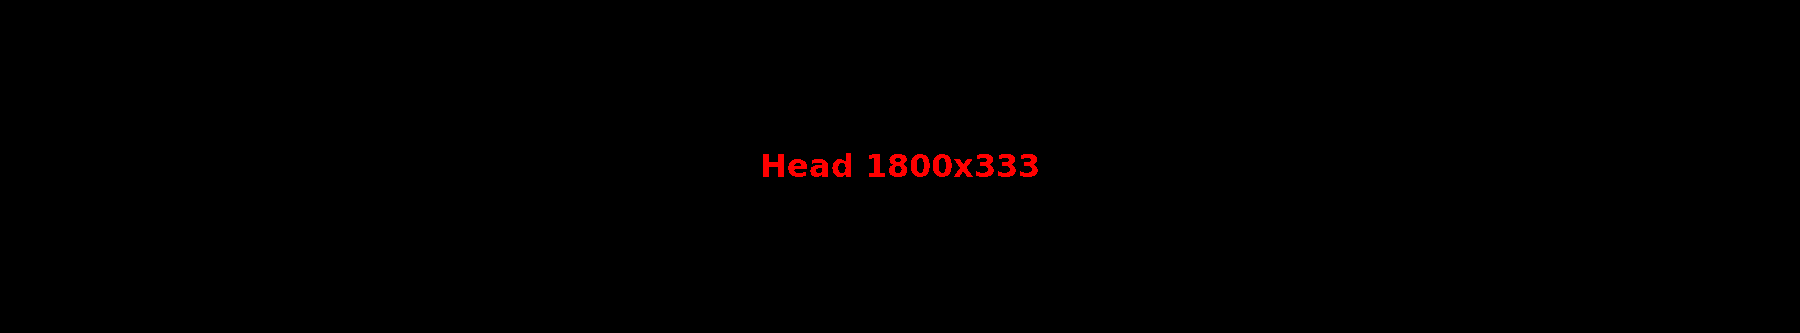
\includegraphics[width=\textwidth]{img/default/head.png}}
%
% Setting up according to choosen EXAM
%
\ifnum \EXAM>0
    \ifnum \EXAM<9
        \newcommand{\DOCUMENTTITLE}{Offensive Security}
        % OSWP
        \ifnum \EXAM=1
            \newcommand{\DOCUMENTSUBTITLE}{OSWP Exam Documentation}
            \newcommand{\VERSION}{v2.0}
        \fi
        % OSCP
        \ifnum \EXAM=2
            \newcommand{\DOCUMENTSUBTITLE}{OSCP Penetration Test Report}
            \newcommand{\VERSION}{v2.0}
        \fi
        % OSWE
        \ifnum \EXAM=3
            \newcommand{\DOCUMENTSUBTITLE}{OSWE Exam Documentation}
            \newcommand{\VERSION}{v1.0}
        \fi
        % OSED
        \ifnum \EXAM=4
            \newcommand{\DOCUMENTSUBTITLE}{OSED Exam Documentation}
            \newcommand{\VERSION}{v1.0}
        \fi
        % OSEP
        \ifnum \EXAM=5
            \newcommand{\DOCUMENTSUBTITLE}{OSEP Exam Documentation}
            \newcommand{\VERSION}{v1.0}
        \fi
        % OSWA
        \ifnum \EXAM=6
            \newcommand{\DOCUMENTSUBTITLE}{OSWA Exam Documentation}
            \newcommand{\VERSION}{v1.0}
        \fi
        % OSDA
        \ifnum \EXAM=7
            \newcommand{\DOCUMENTSUBTITLE}{OSDA Exam Report}
            \newcommand{\VERSION}{v1.0}
        \fi
        % OSMR
        \ifnum \EXAM=8
            \newcommand{\DOCUMENTSUBTITLE}{OSMR Exam Documentation}
            \newcommand{\VERSION}{v1.0}
        \fi
    \else
        % OSEE
        \ifnum \EXAM=42
            \newcommand{\DOCUMENTTITLE}{Offensive Security}
            \newcommand{\DOCUMENTSUBTITLE}{OSEE Exam Documentation}
            \newcommand{\VERSION}{v1.0}
        \else
            % Archive/OSCE
            \ifnum \EXAM=151020
                \newcommand{\DOCUMENTTITLE}{Offensive Security}
                \newcommand{\DOCUMENTSUBTITLE}{OSCE Exam Documentation}
                \newcommand{\VERSION}{v1.0}
            \else
                \newcommand{\DOCUMENTTITLE}{SOMETHING STRANGE HAPPENED}
                \newcommand{\DOCUMENTSUBTITLE}{SOMETHING STRANGE HAPPENED}
                \newcommand{\VERSION}{SOMETHING STRANGE HAPPENED}
            \fi
        \fi
    \fi
\else
    \newcommand{\DOCUMENTTITLE}{SOMETHING STRANGE HAPPENED}
    \newcommand{\DOCUMENTSUBTITLE}{SOMETHING STRANGE HAPPENED}
    \newcommand{\VERSION}{SOMETHING STRANGE HAPPENED}
\fi
%
% metadata
%
\pdfsuppressptexinfo=1
\hypersetup{pdfproducer={\OSID},
    pdfauthor={\MAIL},%
    pdftitle={\DOCUMENTTITLE},%
    pdfsubject={\DOCUMENTSUBTITLE},
    pdfcreator={\NAME},
    pdfborder = {0 0 0}
}
%
%
%
\definecolor{bluekeywords}{rgb}{0.13,0.13,1}
\definecolor{greencomments}{rgb}{0,0.5,0}
\definecolor{redstrings}{rgb}{0.9,0,0}
\definecolor{graynumbers}{rgb}{0.5,0.5,0.5}
\definecolor{osred}{HTML}{A90C1C}
%
% new
%
\newcommand{\sectionbreak}{\clearpage}
%
% renews
%
\renewcommand{\footrulewidth}{0.1pt}
\renewcommand{\headrulewidth}{0pt}
\renewcommand{\sectionmark}[1]{\markboth{#1}{}}
\renewcommand{\familydefault}{\sfdefault}

%
% doc
%
\begin{document}
%
% title page
%
\begin{titlepage}
%
    \begin{center}
        \vspace*{1cm}
        {\fontsize{48}{48}\selectfont \DOCUMENTTITLE}\\
        %
        \vspace{0.5cm}
        {\fontsize{28}{28}\selectfont \DOCUMENTSUBTITLE}\\
        %
        \vspace{0.5cm}
        \textcolor{osred}{\hrule height 2pt}
        \vspace{0.8cm}
        {\fontsize{12}{12}\selectfont \VERSION}\\
        %
        \vspace{0.8cm}
        {\fontsize{16}{16}\selectfont \MAIL}\\
        %
        \vspace{0.8cm}
        {\fontsize{20}{20}\selectfont OSID: \OSID}
        %
        \vspace{0.8cm}
        \vfill
        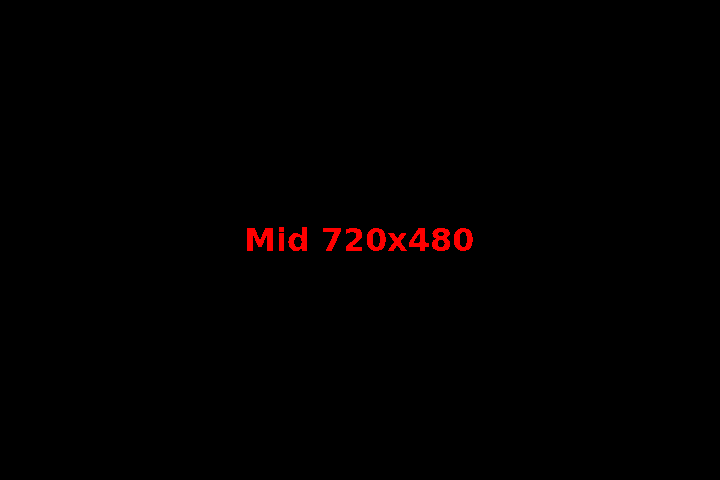
\includegraphics[width=0.7\textwidth]{img/default/mid.png}
        \vfill
        \vspace{0.8cm}
        \textbf{Copyright \copyright \todo[size=\footnotesize]{Put HERE the CORRESPONDING part of the ORIGINAL template}}\vspace{\baselineskip}\linebreak
        %
        %\vspace{0.5cm}
        {No part \todo[size=\footnotesize]{Put HERE the CORRESPONDING part of the ORIGINAL template}}
        %\vspace{0.5cm}
    \end{center}
    \thispagestyle{fancy}
\end{titlepage}
%
% toc
%
\tableofcontents
%
%
%
\ifnum \EXAM>0
    \ifnum \EXAM<9
        % OSWP
        \ifnum \EXAM=1
            % !TeX spellcheck = en_US
% !TeX root = ../../ABCD-OS-XXXXX-Exam-Report.tex
%
%
%
\section{Offensive Security OSWP Exam Documentation}\label{sec:sec1}
%
...
%
%
%
\section{Access Point XYZ}\label{sec:sec2}
%
Listing \ref{lst:sec2-poc} ...\\

\begin{lstlisting}[language=Python,caption={Proof of Concept}, label={lst:sec2-poc}]
    ...
    print('vvvvvvvvvvvvvvvvvvvvvvvvvvvvvvvv-eeeeeeeeeeeeeeeeeeeeeeeeeeeeeeeeeeeeeeeeeee-looooooooooooooooooooooong-striiiiiiiiiiiiiing')
    ...
\end{lstlisting}
%
%
%
\subsection{Proof}\label{sec:sec2-proof}
%
...
%
%
%
\subsection{Screenshots}\label{sec:sec2-screens}
%
Figure \ref{fig:sec2-screen1} ...

\begin{figure}[H]
    \centering
    
\includegraphics[width=\textwidth]{img/assignment1/screen1.png}
    \caption{Screenshot 1}\label{fig:sec2-screen1}
\end{figure}
%
%
%
\subsection{Steps Taken}\label{sec:sec2-steps}
%
...\footnote{Just a footnote.} ... (see section \ref{sec:last-xyz}) ...

\begin{enumerate}
    \item ...
    \item ...
    \item ...
\end{enumerate}
%
%
%
\section{Additional Information not Mentioned Above}\label{sec:last}
%
...
%
%
%
\subsection{...XYZ...}\label{sec:last-xyz}
%
... (see table \ref{tbl:last-xyz}) ...

\begin{table}[H]
    %\begin{tabularx}{\textwidth}{X|l}
    \begin{tabularx}{\textwidth}{l|l}
        \textbf{abc} & \textbf{def} \\
        \hline
        ... & ...\\
    \end{tabularx}
    \caption{XYZ\label{tbl:last-xyz}}
\end{table}


        \fi
        % OSCP
        \ifnum \EXAM=2
            % !TeX spellcheck = en_US
% !TeX root = ../../ABCD-OS-XXXXX-Exam-Report.tex
%
%
%
\section{Offensive Security OSCP Exam Penetration Test Report}\label{sec:sec1}
%
...
%
%
%
\subsection{Introduction}\label{sec:sec1-intro}
%
...
%
%
%
\subsection{Objective(s)}\label{sec:sec1-obj}
%
...
%
%
%
\subsection{Requirements}\label{sec:sec1-req}
%
...
%
%
%
\section{Executive Summary}\label{sec:sec2}
%
...
%
%
%
\subsection{Overall Valuation}\label{sec:sec2-overall}
%
...
%
%
%
\subsection{Recommendations}\label{sec:sec2-recom}
%
...
%
%
%
\section{Methodology}\label{sec:sec3}
%
...

\begin{enumerate}
    \item ...
    \item ...
    \item ...
\end{enumerate}
%
%
%
\subsection{Information Gathering}\label{sec:sec3-infogath}
%
...
%
%
%
\subsection{Enumeration}\label{sec:sec3-enum}
%
...
%
%
%
\subsection{Gaining Access}\label{sec:sec3-gain}
%
...
%
%
%
\subsection{Maintaining Access}\label{sec:sec3-main}
%
...\footnote{Just a footnote.}
%
%
%
\subsection{Cleaning-Up}\label{sec:sec3-clean}
%
...
%
%
%
\section{Independent Challenges / Tasks}\label{sec:sec4}
%
...
%
%
%
\subsection{Target: a.b.c.d}\label{sec:sec4-target1}
%
... (see section \ref{sec:sec4-target1-post}) ...
%
%
%
\subsubsection{Enumeration}\label{sec:sec4-target1-enum}
%
...
%
%
%
\subsubsection{Initial Access / Foothold}\label{sec:sec4-target1-init}
%
...
%
%
%
\subsubsection{Privilege Escalation}\label{sec:sec4-target1-priv}
%
...
%
%
%
\subsubsection{Post Exploitation}\label{sec:sec4-target1-post}
%
Figure \ref{fig:sec4-target1-proof} ...

\begin{figure}[H]
    \centering
    
\includegraphics[width=\textwidth]{img/assignment1/screen1.png}
    \caption{Proof}\label{fig:sec4-target1-proof}
\end{figure}
%
%
%
\subsubsection{Proof of Concept}\label{sec:sec4-target1-poc}
%
Listing \ref{lst:sec4-target1-poc} ...\\

\begin{lstlisting}[language=Python,caption={Proof of Concept}, label={lst:sec4-target1-poc}]
    ...
    print('vvvvvvvvvvvvvvvvvvvvvvvvvvvvvvvv-eeeeeeeeeeeeeeeeeeeeeeeeeeeeeeeeeeeeeeeeeee-looooooooooooooooooooooong-striiiiiiiiiiiiiing')
    ...
\end{lstlisting}
%
%
%
\section{Active Directory Set}\label{sec:sec5}
%
... (see table \ref{tbl:sec5-xyz}) ...

\begin{table}[H]
    %\begin{tabularx}{\textwidth}{X|l}
    \begin{tabularx}{\textwidth}{l|l}
        \textbf{IP} & \textbf{Ports} \\
        \hline
        ... & ...\\
    \end{tabularx}
    \caption{XYZ\label{tbl:sec5-xyz}}
\end{table}
%
%
%
\subsection{Domain Client: a.b.c.d}\label{sec:sec5-client1}
%
...
%
%
%
\subsubsection{Privilege Escalation}\label{sec:sec5-client1-priv}
%
...
%
%
%
\subsubsection{Initial Access / Foothold}\label{sec:sec5-client1-init}
%
...
%
%
%
\subsubsection{Post Exploitation}\label{sec:sec5-client1-post}
%
...
%
%
%
\subsection{Domain Controller: a.b.c.d}\label{sec:sec5-dc1}
%
...
%
%
%
\subsubsection{Initial Access / Foothold}\label{sec:sec5-dc1-init}
%
...
%
%
%
\subsubsection{Privilege Escalation}\label{sec:sec5-dc1-priv}
%
...
%
%
%
\subsubsection{Post Exploitation}\label{sec:sec5-dc1-post}
%
...
%
%
%






%
%
%
\end{document}


        \fi
        % OSWE
        \ifnum \EXAM=3
            % !TeX spellcheck = en_US
% !TeX root = ../../ABCD-OS-XXXXX-Exam-Report.tex
%
%
%
\section{Offensive Security OSWE Exam Documentation}\label{sec:sec1}
%
...

\begin{itemize}
    \item ...
    \item ...
    \item ...
\end{itemize}
%
%
%
\section{Target: a.b.c.d}\label{sec:sec2}
%
...\footnote{Just a footnote.}
%
%
%
\subsection{Proofs: local.txt / proof.txt}\label{sec:sec2-proofs}
%
...
%
%
%
\subsection{Vuln XYZ}\label{sec:sec2-vuln}
%
... (see section \ref{sec:sec2-poc}) ...

%
%
%
\subsection{Proof of Concept}\label{sec:sec2-poc}
Listing \ref{lst:sec2-poc} ...\\

\begin{lstlisting}[language=Python,caption={Proof of Concept}, label={lst:sec2-poc}]
    ...
    print('vvvvvvvvvvvvvvvvvvvvvvvvvvvvvvvv-eeeeeeeeeeeeeeeeeeeeeeeeeeeeeeeeeeeeeeeeeee-looooooooooooooooooooooong-striiiiiiiiiiiiiing')
    ...
\end{lstlisting}
%
%
%
\subsection{Screenshots}\label{sec:sec2-screen1}
%
Figure \ref{fig:sec2-screen1} ...

\begin{figure}[H]
    \centering
    
\includegraphics[width=\textwidth]{img/assignment1/screen1.png}
    \caption{Screenshot 1}\label{fig:sec2-screen1}
\end{figure}
%
%
%
\subsection{Steps Taken}
%
...

\begin{enumerate}
    \item ...
    \item ...
    \item ...
\end{enumerate}
%
%
%
\section{Additional Information not Mentioned Above}\label{sec:last}
%
...
%
%
%
\subsection{...XYZ...}\label{sec:last-xyz}
%
... (see table \ref{tbl:sec5-xyz}) ...

\begin{table}[H]
    %\begin{tabularx}{\textwidth}{X|l}
    \begin{tabularx}{\textwidth}{l|l}
        \textbf{abc} & \textbf{def} \\
        \hline
        ... & ...\\
    \end{tabularx}
    \caption{XYZ\label{tbl:sec5-xyz}}
\end{table}


        \fi
        % OSED
        \ifnum \EXAM=4
            % !TeX spellcheck = en_US
% !TeX root = ../../ABCD-OS-XXXXX-Exam-Report.tex
%
%
%
\section{Offensive Security OSED Exam Documentation}\label{osed-sec:sec1}
%
...~\cite{MitreAttack}
%
%
%
\subsection{Objective(s)}\label{osed-sec:sec1-obj}
%
...
%
%
%
%
\subsection{Requirements}\label{osed-sec:sec1-req}
%
...

\begin{itemize}
    \item ...
    \item ...
    \item ...
\end{itemize}
%
%
%
\section{Executive Summary}\label{osed-sec:sec2}
%
...\footnote{Just a footnote.}
%
%
%
\section{Assignment XYZ}\label{osed-sec:sec3}
%
...
%
%
%
\subsection{Proof: proof.txt}\label{osed-sec:sec3-proof}
%
...
%
%
%
\subsection{Initial Analysis}\label{osed-sec:sec3-init}
%
...
%
%
%
\subsection{Application Analysis}\label{osed-sec:sec3-app}
%
...
%
%
%
\subsection{Vulnerability Discovery}\label{osed-sec:sec3-vuln}
%
...

\begin{enumerate}
    \item ...
    \item ...
    \item ...
\end{enumerate}
%
%
%
\subsection{Exploit Development}\label{osed-sec:sec3-expl}
%
... (see section \ref{osed-sec:sec3-poc}) ...
%
%
%
\subsection{Screenshots}\label{osed-sec:sec3-screens}
%
Figure \ref{osed-fig:sec3-screen1} ...

\begin{figure}[H]
    \centering
    
\includegraphics[width=\textwidth]{img/assignment1/screen1.png}
    \caption{Screenshot 1}\label{osed-fig:sec3-screen1}
\end{figure}
%
%
%
\subsection{Proof of Concept}\label{osed-sec:sec3-poc}
%
Listing \ref{osed-lst:sec3-poc} ...\\

\begin{lstlisting}[language=Python,caption={Proof of Concept}, label={osed-lst:sec3-poc}]
    ...
    print('vvvvvvvvvvvvvvvvvvvvvvvvvvvvvvvv-eeeeeeeeeeeeeeeeeeeeeeeeeeeeeeeeeeeeeeeeeee-looooooooooooooooooooooong-striiiiiiiiiiiiiing')
    ...
\end{lstlisting}
%
%
%
\section{Additional Information not Mentioned Above}\label{osed-sec:last}
%
...
%
%
%
\subsection{...XYZ...}\label{osed-sec:last-xyz}
%
... (see table \ref{osed-tbl:last-xyz}) ...

\begin{table}[H]
    %\begin{tabularx}{\textwidth}{X|l}
    \begin{tabularx}{\textwidth}{l|l}
        \textbf{abc} & \textbf{def} \\
        \hline
        ... & ...\\
    \end{tabularx}
    \caption{XYZ\label{osed-tbl:last-xyz}}
\end{table}
%
%
%
        \fi
        % OSEP
        \ifnum \EXAM=5
            % !TeX spellcheck = en_US
% !TeX root = ../../ABCD-OS-XXXXX-Exam-Report.tex
%
%
%
\section{Offensive Security OSEP Exam Documentation}\label{sec:sec1}
%
...
%
%
%
\subsection{Objective(s)}\label{sec:sec1-obj}
%
...
%
%
%
%
\subsection{Requirements}\label{sec:sec1-req}
%
...

\begin{itemize}
    \item ...
    \item ...
    \item ...
\end{itemize}
%
%
%
\section{Executive Summary}\label{sec:sec2}
%
...\footnote{Just a footnote.}
%
%
%
\section{Target: a.b.c.d}\label{sec:sec3}
%
...
\subsection{Proofs: local.txt / proof.txt / secret.txt}\label{sec:sec3-proofs}
%
...
%
%
%
\subsection{Initial Enumeration}\label{sec:sec3-enum1}
%
...

\begin{enumerate}
    \item ...
    \item ...
    \item ...
\end{enumerate}
%
%
%
\subsection{Exploitation / Gaining Access}\label{sec:sec3-gain}
%
...

Listing \ref{lst:sec3-gain} ...\\

\begin{lstlisting}[language=Python,caption={Proof of Concept}, label={lst:sec3-gain}]
    ...
    print('vvvvvvvvvvvvvvvvvvvvvvvvvvvvvvvv-eeeeeeeeeeeeeeeeeeeeeeeeeeeeeeeeeeeeeeeeeee-looooooooooooooooooooooong-striiiiiiiiiiiiiing')
    ...
\end{lstlisting}
%
%
%
\subsection{Post-Exploitation Enumeration}\label{sec:sec3-enum2}
%
...
%
%
%
\subsection{Local Privilege Escalation}\label{sec:sec3-privescal}
%
... (see section \ref{sec:last}) ...
%
%
%
\subsection{Screenshots}\label{sec:sec3-screen1}
%
Figure \ref{fig:sec3-screen1} ...

\begin{figure}[H]
    \centering
    
\includegraphics[width=\textwidth]{img/assignment1/screen1.png}
    \caption{Screenshot 1}\label{fig:sec3-screen1}
\end{figure}
%
%
%
\section{Additional Information not Mentioned Above}\label{sec:last}
%
...
%
%
%
\subsection{...XYZ...}\label{sec:last-xyz}
%
... (see table \ref{tbl:last-xyz}) ...

\begin{table}[H]
    %\begin{tabularx}{\textwidth}{X|l}
    \begin{tabularx}{\textwidth}{l|l}
        \textbf{abc} & \textbf{def} \\
        \hline
        ... & ...\\
    \end{tabularx}
    \caption{XYZ\label{tbl:last-xyz}}
\end{table}
%
%
%
        \fi
        % OSWA
        \ifnum \EXAM=6
            % !TeX spellcheck = en_US
% !TeX root = ../../ABCD-OS-XXXXX-Exam-Report.tex
%
%
%
\section{Offensive Security OSWA Exam Documentation}\label{oswa-sec:sec1}
%
...

\begin{itemize}
    \item ...
    \item ...
    \item ...
\end{itemize}
%
%
%
\section{Target: a.b.c.d}\label{oswa-sec:sec2}
%
...\footnote{Just a footnote.}
%
%
%
\subsection{Proofs: local.txt / proof.txt}\label{oswa-sec:sec2-proofs}
%
...~\cite{MitreAttack}
%
%
%
\subsection{Vuln XYZ}\label{oswa-sec:sec2-vuln}
%
... (see section \ref{oswa-sec:sec2-poc}) ...

%
%
%
\subsection{Proof of Concept}\label{oswa-sec:sec2-poc}
%
Listing \ref{oswa-lst:sec2-poc} ...\\

\begin{lstlisting}[language=Python,caption={Proof of Concept}, label={oswa-lst:sec2-poc}]
    ...
    print('vvvvvvvvvvvvvvvvvvvvvvvvvvvvvvvv-eeeeeeeeeeeeeeeeeeeeeeeeeeeeeeeeeeeeeeeeeee-looooooooooooooooooooooong-striiiiiiiiiiiiiing')
    ...
\end{lstlisting}
%
%
%
\subsection{Screenshots}\label{oswa-sec:sec2-screens}
%
Figure \ref{oswa-fig:sec2-screen1} ...

\begin{figure}[H]
    \centering
    
\includegraphics[width=\textwidth]{img/assignment1/screen1.png}
    \caption{Screenshot 1}\label{oswa-fig:sec2-screen1}
\end{figure}
%
%
%
\subsection{Steps Taken}\label{oswa-sec:sec2-steps}
%
...

\begin{enumerate}
    \item ...
    \item ...
    \item ...
\end{enumerate}
%
%
%
\section{Additional Information not Mentioned Above}\label{oswa-sec:last}
%
...
%
%
%
\subsection{...XYZ...}\label{oswa-sec:last-xyz}
%
... (see table \ref{oswa-tbl:last-xyz}) ...

\begin{table}[H]
    %\begin{tabularx}{\textwidth}{X|l}
    \begin{tabularx}{\textwidth}{l|l}
        \textbf{abc} & \textbf{def} \\
        \hline
        ... & ...\\
    \end{tabularx}
    \caption{XYZ\label{oswa-tbl:last-xyz}}
\end{table}
%
%
%
        \fi
        % OSDA
        \ifnum \EXAM=7
            % !TeX spellcheck = en_US
% !TeX root = ../../ABCD-OS-XXXXX-Exam-Report.tex
%
%
%
\section{Offensive Security OSDA Exam Report}\label{osda-sec:sec1}
%
...
%
%
%
\subsection{Introduction}\label{osda-sec:sec1-intro}
%
...~\cite{MitreAttack}
%
%
%
\subsection{Objective(s)}\label{osda-sec:sec1-obj}
%
...
%
%
%
\subsection{Requirements}\label{osda-sec:sec1-req}
%
...

\begin{itemize}
    \item ...
    \item ...
    \item ...
\end{itemize}
%
%
%
\section{Executive Summary}\label{osda-sec:sec2}
%
...\footnote{Just a footnote.}
%
%
%
\section{Phases of Attack}\label{osda-sec:sec3}
%
...

\begin{enumerate}
    \item ...
    \item ...
    \item ...
\end{enumerate}
%
%
%
\subsection{Phase One}\label{osda-sec:sec3-phase1}
%
Figure \ref{osda-fig:sec3-phase1-screen1} ...

\begin{figure}[H]
    \centering
    
\includegraphics[width=\textwidth]{img/assignment1/screen1.png}
    \caption{Screenshot 1}\label{osda-fig:sec3-phase1-screen1}
\end{figure}
%
%
%
\subsubsection{Attack XYZ}\label{osda-sec:sec3-phase1-attackxyz}
%
Listing \ref{osda-lst:sec3-phase1-attackxyz} ...\\

\begin{lstlisting}[language=Python,caption={Proof of Concept}, label={osda-lst:sec3-phase1-attackxyz}]
    ...
    print('vvvvvvvvvvvvvvvvvvvvvvvvvvvvvvvv-eeeeeeeeeeeeeeeeeeeeeeeeeeeeeeeeeeeeeeeeeee-looooooooooooooooooooooong-striiiiiiiiiiiiiing')
    ...
\end{lstlisting}
%
%
%
\subsubsection{Persistence}\label{osda-sec:sec3-phase1-pers}
%
...
%
%
%
\subsubsection{Summary}\label{osda-sec:sec3-phase1-sum}
%
... (see section \ref{osda-sec:last}) ...
%
%
%
\subsection{Phase XYZ}\label{osda-sec:sec3-phasexyz}
%
...
%
%
%
\section{Additional Information not Mentioned Above}\label{osda-sec:last}
%
...
%
%
%
\subsection{...XYZ...}\label{osda-sec:last-xyz}
%
... (see table \ref{osda-tbl:last-xyz}) ...

\begin{table}[H]
    %\begin{tabularx}{\textwidth}{X|l}
    \begin{tabularx}{\textwidth}{l|l}
        \textbf{abc} & \textbf{def} \\
        \hline
        ... & ...\\
    \end{tabularx}
    \caption{XYZ\label{osda-tbl:last-xyz}}
\end{table}
%
%
%
        \fi
        % OSMR
        \ifnum \EXAM=8
            % !TeX spellcheck = en_US
% !TeX root = ../../ABCD-OS-XXXXX-Exam-Report.tex
%
%
%
\section{Offensive Security OSMR Exam Documentation}\label{osmr-sec:sec1}
%
...
%
%
%
\subsection{Objective(s)}\label{osmr-sec:sec1-obj}
%
...~\cite{MitreAttack}
%
%
%
\subsection{Requirements}\label{osmr-sec:sec1-req}
%
...

\begin{itemize}
    \item ...
    \item ...
    \item ...
\end{itemize}
%
%
%
\section{Executive Summary}\label{osmr-sec:sec2}
%
...\footnote{Just a footnote.}
%
%
%
\section{Assignment XYZ}\label{osmr-sec:sec3}
%
...
%
%
%
\subsection{Proofs: local.txt / proof.txt / secret.txt}\label{osmr-sec:sec3-proofs}
%
...
%
%
%
\subsection{Initial Analysis}\label{osmr-sec:sec3-init}
%
...
%
%
%
\subsection{Vulnerability Discovery}\label{osmr-sec:sec3-vuln}
%
...

\begin{enumerate}
    \item ...
    \item ...
    \item ...
\end{enumerate}
%
%
%
\subsection{Exploit or Bypass Development}\label{osmr-sec:sec3-expl}
%
... (see section \ref{osmr-sec:sec3-poc}) ...
%
%
%
\subsection{Screenshots}\label{osmr-sec:sec3-screens}
%
Figure \ref{osmr-fig:sec3-screen1} ...

\begin{figure}[H]
    \centering
    
\includegraphics[width=\textwidth]{img/assignment1/screen1.png}
    \caption{Screenshot 1}\label{osmr-fig:sec3-screen1}
\end{figure}
%
%
%
\subsection{Proof of Concept}\label{osmr-sec:sec3-poc}
%
Listing \ref{osmr-lst:sec3-poc} ...\\

\begin{lstlisting}[language=Python,caption={Proof of Concept}, label={osmr-lst:sec3-poc}]
    ...
    print('vvvvvvvvvvvvvvvvvvvvvvvvvvvvvvvv-eeeeeeeeeeeeeeeeeeeeeeeeeeeeeeeeeeeeeeeeeee-looooooooooooooooooooooong-striiiiiiiiiiiiiing')
    ...
\end{lstlisting}
%
%
%
\section{Additional Information not Mentioned Above}\label{osmr-sec:last}
%
...
%
%
%
\subsection{...XYZ...}\label{osmr-sec:last-xyz}
%
... (see table \ref{osmr-tbl:last-xyz}) ...

\begin{table}[H]
    %\begin{tabularx}{\textwidth}{X|l}
    \begin{tabularx}{\textwidth}{l|l}
        \textbf{abc} & \textbf{def} \\
        \hline
        ... & ...\\
    \end{tabularx}
    \caption{XYZ\label{osmr-tbl:last-xyz}}
\end{table}
%
%
%
        \fi
    \else
         % OSEE
        \ifnum \EXAM=42
            % !TeX spellcheck = en_US
% !TeX root = ../../ABCD-OS-XXXXX-Exam-Report.tex
%
%
%
\section{Offensive Security OSEE Exam Documentation}\label{osee-sec:sec1}
%
...

\begin{itemize}
    \item ...
    \item ...
    \item ...
\end{itemize}
%
%
%
\section{Target: a.b.c.d}\label{osee-sec:sec2}
%
...\footnote{Just a footnote.}
%
%
%
\subsection{Proof: proof.txt}\label{osee-sec:sec2-proof}
%
...
%
%
%
\subsection{ROP Chain(s) in Detail}\label{osee-sec:sec2-rop}
%
...
%
%
%
\subsection{Proof of Concept}\label{osee-sec:sec2-poc}
%
Listing \ref{osee-lst:sec2-poc} ...\\

\begin{lstlisting}[language=Python,caption={Proof of Concept}, label={osee-lst:sec2-poc}]
    ...
    print('vvvvvvvvvvvvvvvvvvvvvvvvvvvvvvvv-eeeeeeeeeeeeeeeeeeeeeeeeeeeeeeeeeeeeeeeeeee-looooooooooooooooooooooong-striiiiiiiiiiiiiing')
    ...
\end{lstlisting}
%
%
%
\subsection{Screenshots}\label{osee-sec:sec2-screens}
%
Figure \ref{osee-fig:sec2-screen1} ...

\begin{figure}[H]
    \centering
    
\includegraphics[width=\textwidth]{img/assignment1/screen1.png}
    \caption{Screenshot 1}\label{osee-fig:sec2-screen1}
\end{figure}
%
%
%
\subsection{Steps Taken}\label{osee-sec:sec2-steps}
%
...

\begin{enumerate}
    \item ...
    \item ...
    \item ...
\end{enumerate}
%
%
%
\section{Target: XYZ}\label{osee-sec:sec3}
%
...
%
%
%
\subsection{Proof: proof.txt}\label{osee-sec:sec3-proof}
%
...
%
%
%
\subsection{Shellcode in Detail}\label{osee-sec:sec3-asm}
%
... (see section \ref{osee-sec:sec3-poc}) ...
%
%
%
\subsection{Proof of Concept}\label{osee-sec:sec3-poc}
%
...
%
%
%
\subsection{Screenshots}\label{osee-sec:sec3-screens}
%
...
%
%
%
\subsection{Steps Taken}\label{osee-sec:sec3-steps}
%
...
%
%
%
\section{Additional Information not Mentioned Above}\label{osee-sec:last}
%
...
%
%
%
\subsection{...XYZ...}\label{osee-sec:last-xyz}
%
... (see table \ref{osee-tbl:last-xyz}) ...

\begin{table}[H]
    %\begin{tabularx}{\textwidth}{X|l}
    \begin{tabularx}{\textwidth}{l|l}
        \textbf{abc} & \textbf{def} \\
        \hline
        ... & ...\\
    \end{tabularx}
    \caption{XYZ\label{osee-tbl:last-xyz}}
\end{table}
%
%
%
        \else
            % Archive/OSCE
            \ifnum \EXAM=151020
                % !TeX spellcheck = en_US
% !TeX root = ../../../ABCD-OS-XXXXX-Exam-Report.tex
%
%
%
\section{Offensive Security OSCE Exam Documentation}\label{osce-sec:sec1}
%
...

\begin{itemize}
    \item ...
    \item ...
    \item ...
\end{itemize}
%
%
%
\section{Target: a.b.c.d}\label{osce-sec:sec2}
%
...\footnote{Just a footnote.}
%
%
%
\subsection{Proof: proof.txt}\label{osce-sec:sec2-proof}
%
...
%
%
%
\subsection{Vulnerable Command}\label{osce-sec:sec2-vulncmd}
%
...
%
%
%
\subsection{Vulnerability Identification}\label{osce-sec:sec2-vulnid}
%
...
%
%
%
\subsection{Proof of Concept}\label{osce-sec:sec2-poc}
%
Listing \ref{osce-lst:sec2-poc} ...\\

\begin{lstlisting}[language=Python,caption={Proof of Concept}, label={osce-lst:sec2-poc}]
    ...
    print('vvvvvvvvvvvvvvvvvvvvvvvvvvvvvvvv-eeeeeeeeeeeeeeeeeeeeeeeeeeeeeeeeeeeeeeeeeee-looooooooooooooooooooooong-striiiiiiiiiiiiiing')
    ...
\end{lstlisting}
%
%
%
\subsection{Steps Taken}\label{osce-sec:sec2-steps}
%
...

\begin{enumerate}
    \item ...
    \item ...
    \item ...
\end{enumerate}
%
%
%
\section{Target: 1.2.3.4}\label{osce-sec:sec3}
%
...
%
%
%
\subsection{Proof: proof.txt}\label{osce-sec:sec3-proof}
%
...
%
%
%
\subsection{Vulnerable Code}\label{osce-sec:sec3-vulncode}
%
... (see section \ref{osce-sec:sec3-poc}) ...
%
%
%
\subsection{Privilege Escalation}\label{osce-sec:sec3-privescal}
%
...
%
%
%
\subsection{Proof of Concept}\label{osce-sec:sec3-poc}
%
...
%
%
%
\subsection{Screenshots}\label{osce-sec:sec3-screens}
%
Figure \ref{osce-fig:sec3-screen1} ...

\begin{figure}[H]
    \centering
    
\includegraphics[width=\textwidth]{img/assignment1/screen1.png}
    \caption{Screenshot 1}\label{osce-fig:sec3-screen1}
\end{figure}
%
%
%
\subsection{Steps Taken}\label{osce-sec:sec3-steps}
%
...
%
%
%
\section{Target: XYZ}\label{osce-sec:sec4}
%
...
%
%
%
\subsection{Screenshots}\label{osce-sec:sec4-screens}
%
...
%
%
%
\subsection{Steps Taken}\label{osce-sec:sec4-steps}
%
...
%
%
%
\section{Target: ABC}\label{osce-sec:sec5}
%
...
%
%
%
\subsection{Proof of Concept}\label{osce-sec:sec5-poc}
%
...
%
%
%
\subsection{Screenshots}\label{osce-sec:sec5-screens}
%
...
%
%
%
\subsection{Steps Taken}\label{osce-sec:sec5-steps}
%
...
%
%
%
\section{Additional Information not Mentioned Above}\label{osce-sec:last}
%
...
%
%
%
\subsection{...XYZ...}\label{osce-sec:last-xyz}
%
... (see table \ref{osce-tbl:last-xyz}) ...

\begin{table}[H]
    %\begin{tabularx}{\textwidth}{X|l}
    \begin{tabularx}{\textwidth}{l|l}
        \textbf{abc} & \textbf{def} \\
        \hline
        ... & ...\\
    \end{tabularx}
    \caption{XYZ\label{osce-tbl:last-xyz}}
\end{table}
%
%
%
            \else
                % !TeX spellcheck = en_US
% !TeX root = ../ABCD-OS-XXXXX-Exam-Report.tex
%
%
%
\todo[inline]{You have to set the corresponding number for your exm in ABCD-OS-XXXXX-Exam-Report.tex}
            \fi
        \fi
    \fi
\else
    % !TeX spellcheck = en_US
% !TeX root = ../ABCD-OS-XXXXX-Exam-Report.tex
%
%
%
\todo[inline]{You have to set the corresponding number for your exm in ABCD-OS-XXXXX-Exam-Report.tex}
\fi
%
%
%
\end{document}

